\section{Le \textsf{NoSQL}}

Le NoSQL signifiant littéralement « \textsf{Not only SQL} » est une
dénomination désignant une catégorie de gestionnaire de bases de
données massives. Ces gestionnaires \textsf{NoSQL} optent pour la
simplicité au détriment de certaines fonctionnalités classiques des
\textsf{SGBD}\footnote{Système de Gestion de Base de Données}
relationnels pour plus de performance et une meilleure
scalabilité. Cependant, notons que les \textsf{SGBD} non-relationnels
sont plus anciens que les \textsf{SGBD} relationnels et sont répandus
sur les mainframes et les logiciels d'annuaire. Par exemple, le
stockage d'information à l'aide de tableaux associatifs existe depuis
le début de l'histoire des bases de données, en 1970.  \\ \\ Les
\textsf{SGBD} non-relationnels ont connu une nouvelle jeunesse avec le
\textsf{NoSQL} dans le domaine des services \textsf{Internet}. Ce
retour aux non-relationnels est essentiellement motivé par les
nouvelles demandes en rapport avec les sites web de grande audience
apparus dans les années 2000. La plupart des logiciels \textsf{NoSQL}
sont destinés à être utilisés dans les dispositifs en répartition de
charge des grands services \textsf{Internet}. Ceci dit que le
\textsf{NoSQL} a pour ambition d'apporter une solution face à la
montée en charges des bases de données dans le monde de
l'\textsf{Internet}.  \\ \\ La conférence meet-up\index{Meet-up 2009 à
  San-Francisco} de 2009 à \textsf{San-Francisco} est considérée comme
l'inauguration de la communauté des développeurs de logiciels
\textsf{NoSQL}. Cependant et comme le souligne \textsf{wikipedia}, les
leaders de la communauté \textsf{NoSQL} sont des \textsf{start-up} de
développeurs critiqués de ne pas avoir les moyens d'acheter les
\textsf{SGBD} de Oracle\cite{wikiNoSQL}. Il est important de noter que
la communauté \textsf{NoSQL} a effectivement mis en place des produits
capables de manipuler de très grandes quantités de données qui se
mesurent en centaines de \texttt{Téraoctets} et offrent une meilleure
scalabilité mais force est de remarquer que les solutions
\textsf{NoSQL} sont seulement adaptées pour certains besoins comme
ceux des applications \texttt{Web 2.0}.  \\\\ On reproche à la
mouvance \textsf{NoSQL} de sacrifier le principe
\textsf{ACID}\footnote{voir annexe \ref{acid}} donc de ne pas pouvoir
garantir une grande sûreté dans l'accès aux données. Cependant une
nouvelle mouvance, le \textsf{NewSQL}, tente de conserver la
structure classique en colonnes tout en faisant appel à différents
procédés dans le but de conserver la rapidité même sur de larges
volumes\cite{newSQL}.

\subsection{Les différents types de bases de données \textsf{NoSQL}} 
 
Dans la mouvance \textsf{NoSQL}, les données sont représentées de
diverses manières. Ainsi définit-on des catégories de gestionnaire
\textsf{NoSQL} en fonction de la manière de représenter les données.
\\\\ \textsf{Clé - valeur}\index{NoSQL!Orienté clé - valeur}: La
représentation la plus simple. Cette structure est très adaptée à la
gestion de caches ou pour fournir un accès rapide aux
informations. Comme pour une table de hashage, chaque clé est associée
à une seule valeur dont elle ne connaît pas la structure. Ce postulat
permet en général d’atteindre des performances bien supérieures dans
la mesure où les lectures et écritures sont réduites à un accès disque
simple. Cette catégorie trouve sa légitimité dans le constat que les
applications présentent de nombreux accès à la base de données qui ne
sont que de simples lectures ou écritures à partir d’un
identifiant\cite{cleValeur}.  \\\\ {\sf Document}:
Ajoute\index{NoSQL!Orienté document} au modèle clé-valeur,
l’association d’une valeur à structure non plane, c’est-à-dire qui
nécessiterait un ensemble de jointures en logique relationnelle.  la
valeur est sous la forme d'un document contenant des données
organisées de manière hiérarchique à l’image de ce que permettent
\textsf{XML} ou \textsf{JSON}.  \\\\ {\sf Colonne}\index{NoSQL!Orienté
  Colonne}: Autre évolution du modèle clé-valeur, il permet de
disposer d'un très grand nombre de valeurs sur une même ligne,
permettant ainsi de stocker les relations de type one-to-many. Les
lignes peuvent avoir des types de colonnes différents et également des
nombres de colonnes différents. On dispose également d'une hiérarchie
entre les colonnes. Contrairement au système Clé-Valeur, celui-ci
permet d’effectuer des requêtes par clé.  \\\\ {\sf
  Graphe}\index{NoSQL!Orienté graphe}: très adapté pour la modélisation, le
stockage et la manipulation des relations non-triviales ou variables
entre les données. Un cas classique d'utilisation de cette catégorie
est le stockage des informations des réseaux sociaux. Ces informations
sont difficilement modélisables dans une base de données
relationnelle.  \\ \\ {\color{red} {\sf La représentation utilisée par
    cubeLaBRI}: encore inconnu} \\ \\ \textsf{D'autres
  représentations}: \textsf{Xml}, \textsf{bases de données objet},
\textsf{les bases de données hiérarchiques ou encore les datagrids}
...

\subsection{Quelques exemples de \textsf{NoSQL}}

Les logiciels n'utilisant pas le modèle relationnel classique est en
nombre croissant et les exemples de \textsf{NoSQL} ci-dessous correspondent à ceux en open source, assez connus exceptés
\textsf{BigTable} et \textsf{cubeLaBRI} qui sont propriétaires.
\\\\ {\sf MongoDB}: MongoDB est une base de données « \textsf{orientée
    document} » totalement open-source développée en
\textsf{C++}. MongoDB stocke les données sous forme de \textsf{JSON}
dont la structure reste libre et dynamique.  En effet, aucun schéma de
\textsf{BDD}\footnote{Base De Données} à respecter n'est défini à
l'avance.\cite{mongoDB} \\\\ \textsf{Cassandra}: \index{Cassandra} une
solution \textsf{NoSQL} d’\textsf{Apache}.  C’est une \textsf{BDD} orientée colonnes
qui se veut être hautement extensible. C’est-à-dire qu’il est très
simple d’ajouter ou d’enlever - c’est rare - un nœud du
cluster. D’abord développé par \textsf{Facebook}, le code source est devenu
« \textsf{Open-Source} » et repris par la fondation \textsf{Apache}\cite{cassandra}.  La
technologie est encore peu maîtrisée mais elles revienne régulièrement
dans l’actualité du fait des régulières annonces de migrations de
quelques entreprises \textsf{web} renommées\cite{cassandra2}.
\\\\ \textsf{BigTable}: \index{Bigtable} système de gestion de base de
données propriétaire, développé et exploité par Google qui ne
distribue pas sa base de données mais propose une utilisation publique
via sa plateforme d'application \textsf{Google App Engine}. Son
développement a commencé en $2004$ et est aujourd'hui utilisé par les
applications \textsf{Google} telles que \textsf{Google Earth},
\textsf{Blogger.com}, \textsf{Google Code hosting}, \textsf{YouTube},
\textsf{Gmail} ... D'autres projets libres tels que \textsf{HBase},
\textsf{Cassandra} ou \textsf{Hypertable} s'en sont
inspirés.\cite{bigtable} \\\\ {\color{red} \textsf{cubeLaBRI}: en
  attente de documentation.}

\section{\textsf{SQL} vs \textsf{NoSQL}}
Il serait tout à fait légitime de penser que le 
\textsf{NoSQL} soit là pour remplacer les \textsf{BDDR}
classiques. Mais ceci est difficilement imaginable de
nos jours. L’intérêt pour le \textsf{NoSQL} s'est considérablement
accru à l'issu des annonces d’adoption de ces technologies par les 
grands acteurs d'\textsf{Internet} tels 
\textsf{Google} et \textsf{Facebook} qui se sont multipliées. Ces acteurs
n'ont pas pour autant abandonné \textsf{BDDR}. \textsf{Google} et 
\textsf{Facebook} utilisent \textsf{MySQL}\cite{mysqlcustomers}.
\\
\\
Ci-dessous quelques traitements auxquels le modèle relationnel
classique ne répond pas et qui pourrait motiver le recours aux
technologies \textsf{NoSQL}\index{Limites du \textsf{SQL}}:

%% \paragraph{Indexation d'une quantité de documents:}
%% Un problème se pose quant à l'indexation d'une quantité importante de
%% données. Par exemple pour le \textsf{SGBD} \textsf{SQL Server}, la
%% version $2008$ supporte au plus $999$ indexes et chaque index, chaque
%% index peut couvrir au maximum 16 colonnes et la somme des tailles des
%% colonnes couvertes ne doit pas excéder $900\ octets$\cite{SQLserver}

\paragraph{Environnement distribué:} pour faire face à des volumes importants 
de données, il est possible de les repartir sur différentes machines physiques. 
Pour avoir plusieurs points d'accès aux données, il est nécessaire de les dupliquer
sur différents serveurs. Toutes ces opérations constituent en la mise en place d'un 
environnement distribué. Les \textsf{SGBDR} classiques montrent des limites dans un 
environnement distribué. Ces {SGBD} ne sont pas destinés à fonctionner dans un
environnement à données reparties du fait de l'opération de jointure
qui est difficilement réalisable entre des tables réparties sur des systèmes différents\cite{RickCattell}.
Les \textsf{SGBDR} classiques effectuent également des opérations impliquant de la distribution des données
mais ces opérations ne sont pas du type « \textit{shared nothing} ». Les coeurs et les processus impliqués
dans ces opérations se partagent mutuellement la \textsf{RAM} et l'espace disque mémoire.

\paragraph{Données à structure dynamique et libre:} les 
\textsf{BDDR} classiques prévoient un schéma statique à 
l'avance. Le schéma est organisé en tables de données où les lignes
contiennent les mêmes types et nombre de colonnes. Celles-ci n'offrent
donc pas un environnement dynamique pour les enregistrements. Aussi
les \textsf{SGBDR} fonctionnent avec des données structurées
organisables en tables.  Ce n'est pas le cas avec des données non
structurées, telles les données de traitement de texte et les images
\cite{NealLeavitt}.

\paragraph{Réécritures fréquentes:}  en effet, les \textsf{SGBDR} classiques en générale
appliquent la consistance forte et ce grâce aux propriétés \textsf{ACID}. 
Ces opérations sont à l'origine d'\textit{overhead} 
et sont appliquées même pour les opérations simples d'écriture dans la base. Ceci diminuera
considérablement la performance en cas de réécritures fréquentes des données même pour
les opérations simples.
Les \textsf{BDDR} mettent en avant un système d'indexation très évolué. L'utilisation
d'index est plutôt conseillée pour les systèmes où l'accès en écriture est
beaucoup plus important que celui en écriture. Tout ceci laisse penser que le modèle relationnel
classique prévoit plus de lectures que d'écritures. 

\paragraph{Extensibilité de la base:} comme signaler à la section \ref{carac}, 
la scalabilité horizontale qui est l'une des caractéristiques principales 
des solutions \textsf{NoSQL}, offre la possibilité 
d'ajouter des nœuds au cluster pour gagner en performance. Les \textsf{SGBDR} classiques 
n'ont pas cette propriété de scalabilité horizontale.
\\ 
\\ 
L'extensibilité requise, la grande quantité de données
et les mises à jour massives rendent le modèle relationnel inefficace, ce qui a
obligé à trouver un nouveau modèle. Cependant il est important de prendre en
considération quelques aspects au risque d'une mauvaise utilisation. «
L'intérêt d'une base de données \textsf{NoSQL} pour un projet ne
dépend pas du volume de données qu'elle aura à manipuler. Le choix de
son utilisation doit être basé sur la préférence d’un mode de
représentation et non sur une forte volumétrie
»\cite{NoSQLeurope}. Il ne s’agit donc pas d’une solution
miracle pour tout type de stockage de données.  La tentative de
reproduire dans une base de données \textsf{NoSQL} une représentation
ou un comportement habituellement offert par la représentation en tables
n'aboutira pas à une solution plus efficace car l'architecture des 
\textsf{SGBDR} y est exclusivement destinée.
%Dan McCreary a également convenu avec Michael Stonebraker que les
%utilisateurs NoSQL ne partagent pas un langage de requête unifiée, ce
%qui va ralentir l'adoption de NoSQL\cite{SergeLeblal}.
\\
\\
À présent, je vais attirer l'attention sur une différence fondamentale
entre ces deux familles de gestionnaires de données. Elles n'ont pas
la même conception de la gestion des données. Le \textsf{SQL} impose
un format de stockage le plus explicite possible à l'utilisateur pour
permettre au gestionnaire d'avoir la maîtrise totale des données
stockées afin d'en assurer l'intégrité. Le gestionnaire \textsf{SQL}
ne se contente pas uniquement de répondre aux requêtes. Il effectue
d'autres opérations qui consistent en l'entretien de la base à l'image
de \textsf{MySQL} dont 96\% des cycles machines sont de
l'\textit{overhead}. Le \textsf{NoSQL} vise à éviter les opérations
d'\textit{overhead} afin de consacrer toutes les ressources machines
aux seuls traitements des requêtes pour être plus rapide. Cependant
la cohérence dans la \textsf{BDD} nécessite beaucoup d'apport
extérieur pour pallier à la très grande souplesse du système.  Une
illustration de cette différence philosophique entre les
deux familles de gestionnaires est la suivante:
\begin {figure}[H]
       \centering
        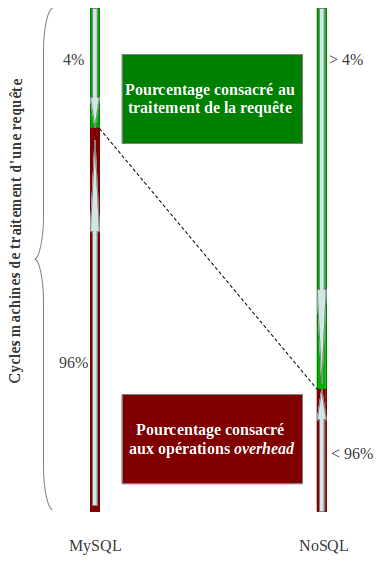
\includegraphics[scale=0.3]{\DIR/img/SQLvsNoSQL.png}	
        \caption{Répartitions des cycles machines \textsf{SQL} et \textsf{NoSQL}}
	\label{sqlvsnoql}
  \end {figure}    
\noindent
Toujours en quête de performance et comme mentionné à la section \ref{carac}, 
le \textsf{NoSQL} a renoncé à de la « \textsf{consistance forte} » pour de la « \textsf{consistance éventuelle} ». Il justifie ce choix par le théorème de \textsf{CAP} pendant que les \textsf{SGBDR} défendent systématiquement toutes les propriétés \textsf{ACID} dont la « \textsf{consistance forte} ». Ceci n'est pas sans compromis, notamment 
pour la reprise sur erreurs. 
\textsf{Michael Stonebraker} explique clairement sur 8 cas d'erreur,  
les enjeux du choix
des propriétés \textsf{CAP}\cite{MichaelStonebraker2}. Je me limiterai seulement à
3 cas d'erreur. Le but étant de mettre en relief les limites d'une « \textsf{consistance éventuelle} »
et d'exhiber deux situations qui rendent impossible la propriété \textsf{A} de \textsf{CAP} défendue par la mouvance \textsf{NoSQL}.
%===========================================================
%     Illustration enjeux du choix de AP dans CAP
%===========================================================
\def\exempleA{We assume a typical hardware model of a
collection of local processing and storage nodes assembled into a cluster using LAN networking.
The clusters, in turn, are wired together using WAN networking.
Let’s start with a discussion of what causes errors in databases:}

\def\exemple{Dans l'illustration qu'il a utilisé, \textsf{Michael Stonebraker} a considéré un ensemble de clusters interconnectés via un réseau \textsf{WAN}. 
Les nœuds à l'intérieur d'un cluster utilisent le \textsf{LAN} pour échanger. Ci-dessous trois cas d'erreur possibles:}

\def\casaA{Application errors. The application performed one or more incorrect updates. Generally, this is
not discovered for minutes to hours thereafter. The database must be
backed up to a point before the offending transaction(s), and
subsequent activity redone.}

\def\casa{Erreur au niveau de la couche application. Une application effectue une ou plusieurs mises à jour incorrectes. De telles erreurs ne sont généralement pas détectées dans les minutes qui suivent afin de revenir sur une version précédente de la base avant les mises à jour incorrectes.}

\def\casbA{Repeatable DBMS errors. The DBMS crashed at a processing node. Executing the same
transaction on a processing node with a replica will cause the backup
to crash. These errors have been termed Bohr bugs.}

\def\casb{Les erreurs reproductibles. Par exemple, une transaction fait planter le serveur principal. 
La même transaction fait tomber tous les autres serveurs copies qui vont servir de relais. 
Ces erreurs sont connues sous le nom de « \textsf{Bohr bugs} ».}

\def\cascA{\sf A disaster. The local cluster is wiped out by a flood, earthquake, etc. The cluster no longer exists.}

\def\casc{\sf Une catastrophe. Un cluster local est entièrement détruit.}

\def\commentA{First, note that errors 1 and 2 will cause problems with any high availability scheme. In these two
scenarios, there is no way to keep going; i.e., availability is
impossible to achieve. Also, replica consistency is meaningless; the
current DBMS state is simply wrong. Error 7 will only be recoverable
if a local transaction is only committed after the assurance that the
transaction has been received by another WAN-connected cluster. Few
application builders are willing to accept this kind of
latency. Hence, eventual consistency cannot be guaranteed, because a
transaction may be completely lost if a disaster occurs at a local
cluster before the transaction has been successfully forwarded
elsewhere. Put differently, the application designer chooses to suffer
data loss when a rare event (such as a disaster) occurs, because the
performance penalty for avoiding it is too high.}

\def\comment{Les deux premiers cas d'erreur conduisent la base dans un état incohérent. Ils affectent la disponibilité des données. Dans de telles situations, il est impossible de garantir la disponibilité des données même après avoir renoncé à de la consistance forte. Le troisième cas d'erreur montre les limites de
la consistance éventuelle. Les données ne pourront être récupérées que
si la transaction a été propagée sur un autre cluster avant la
catastrophe. Le temps de latence imposé par la consistance éventuelle
entre les mises à jour est donc problématique.}

\begin{center}
\begin{tabular}{p{1.7cm} p{12cm}}
\multicolumn{2}{p{14cm}}{\sf \exemple}\\&\\  
{\bf Cas 1} & \textsf{\casa}\\~&~\\ {\bf Cas 2}
& \textsf{\casb}\\~&~\\ {\bf Cas 3} & \textsf{\casc}\\
\end{tabular}
\end{center}
\noindent \comment
\\
\\
Pour finir, un paramètre à prendre en compte et pour ainsi reprendre la pensée de \textsf{Ted Dziuba},
est que contrairement aux solutions \textsf{NoSQL}, les \textsf{SGBDR} sont matures et ont par conséquent 
``une liste de limitations et de bugs connus''\cite{DieNosql}. L'utilisateur d'une \textsf{SGBDR} classique 
est plus ou moins rassuré parce qu'il sait à quoi s'en tenir. 


\section{Échange entre \textsf{SQL} et \textsf{NoSQL}}
Pour profiter des performances d'un \textsf{NoSQL}, il est essentiel
de définir à l'avance la nature et la représentation faite des données.
L'utilité et le choix du \textsf{NoSQL} doit principalement
réposer de la représentation des données. Adopter le \textsf{NoSQL} à
cause de la volumétrie ne garantit pas la performance et surtout la 
base perd l'intégrité qu'offre le modèle rélationnel.  
\\ 
\\ 
Les « \textsf{NoSQL} » offrent une autre façon
de représenter les données pour faciliter les accès et mises à jour des
données afin de gagner en performance. Le \textsf{NoSQL} n'est pas 
là pour remplacer systématiquement le  \textsf{SQL}. Pour la gestion des données 
organisée en tables, la structure des \textsf{SGBDR} y est exclusivement
dédiée. Cependant certaines solutions \textsf{NoSQL}, à l'image de \textsf{MongoDB}, ont
exhibé une charte de correspondance entre leurs composants et les composants \textsf{BDDR} 
\footnote{Database, Table, Index, colonne, clé
  primaire ...}. \textsf{MongoDB} a également mis
en place une charte de traduction requête \textsf{SQL} / requête
\textsf{MongoDB}.
\\
\\
\textsf{SQL} d'une part, \textsf{NoSQL} d'autre part, l'un n'exclut pas l'autre.
Tout dépend de l'usage qu'on compte en faire ou du profit qu'on
souhaite en tirer. Pour profiter à la fois du \textsf{NoSQL} et du \textsf{SQL}, il est très commun
de les faire cohabiter et de stocker
les données dans l'un ou dans l'autre en fonction des caractéristiques de 
celles-ci. C'est ce que fait d'ailleurs \textsf{Google} qui
même après avoir mis en place sa solution
propriétaire \textsf{BigTable} utilise \textsf{MySQL}
notamment pour son programme publicitaire \textsf{AdWords}, sa
principale source de revenue, et qui utilise d'énormes quantités de
données. Cependant imaginer un protocole d'échange entre \textsf{SQL}
et \textsf{NoSQL} peut s'avérer très fastidieux dans la mesure où les
deux conçoivent les données très différemment.
\\
\\
Il existe une solution \textsf{Open Source} permettant des échanges
\textsf{SQL}/\textsf{NoSqL}: \textsf{Sqoop} ou « SQL To Hadoop
». \textsf{Hadoop}\index{Sqoop} est un assemblage de plusieurs
sous-projet avec à la base un système de
fichier \textsf{HDFS}\footnote{Hadoop Distributed File System}
et \textsf{HBASE} pour le stockage. Développé en \textsf{java}, sous
la direction de la fondation \textsf{Apache} et destiné aux
applications distribuées, sa structure de stockage \textsf{HBASE} est
un x\textsf{NoSQL} orienté colonnes. \textsf{Sqoop} charge
une table ou toute la base en système de fichiers \textsf{HDFS} en
fonction des options d'importation spécifiées et génère aussi des
classes \textsf{java} correspondantes aux tables de la bases, ainsi
que des objets correspondants aux lignes pour permettre d'interagir
avec les données importées.
\begin {figure}[H]
       \centering
        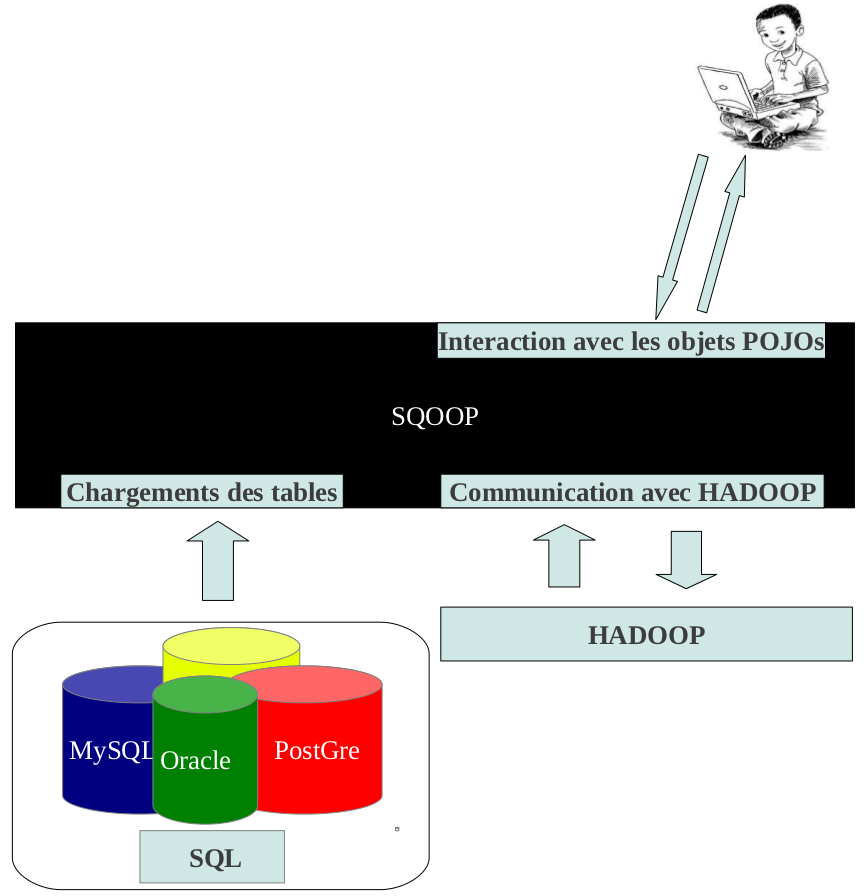
\includegraphics[scale=0.2]{\DIR/img/sqoop.png}	
        \caption{Fonctionnement de \textsf{SQOOP}}
	\label{sqoop}
  \end {figure}    
\noindent
Mise à part \textsf{Sqoop} qui est une solution pour \textsf{Hadoop}
d'échange avec le \textsf{SQL}, le framework
\textsf{spring} intègre des modules \textsf{Data access}\cite{springsource} permettant 
de faire persister des objets \textsf{POJO}\footnote{Acronyme de \textsf{P}lain \textsf{O}ld \textsf{J}ava \textsf{O}bject désignant les objets java simples n'héritant d'aucune classe et n'implémentant aucune interface } dans des \textsf{BDD NoSQL}. 
En exemple, le module \textsf{Spring Data MongoDB} permet de faire persister
les données dans \textsf{MongoDB}. Avec \textsf{spring} il est alors possible
d'effectuer une échange en deux temps:
\begin{enumerate}
\item D'abord transformer les données dans la \textsf{BDDR} en des objets 
      \textsf{POJO} par le biais de module déjà existant
      comme \textsf{hibernate, toplink, iBatis}...
\item Puis faire persister les objets \textsf{POJO} dans la base \textsf{NoSQL} par le biais du module 
      \textsf{Data access} dédié.    
\end{enumerate} 
Cependant il faut changer de module \textsf{Data access} à chaque fois
qu'il faut changer de \textsf{BDD NoSQL}. Il est difficile de mettre
en place une standardisation des interfaces dans la mesure où
chaque \textsf{BDD NoSQL} vient avec son propre langage de requête.
\begin {figure}[H]
       \centering
        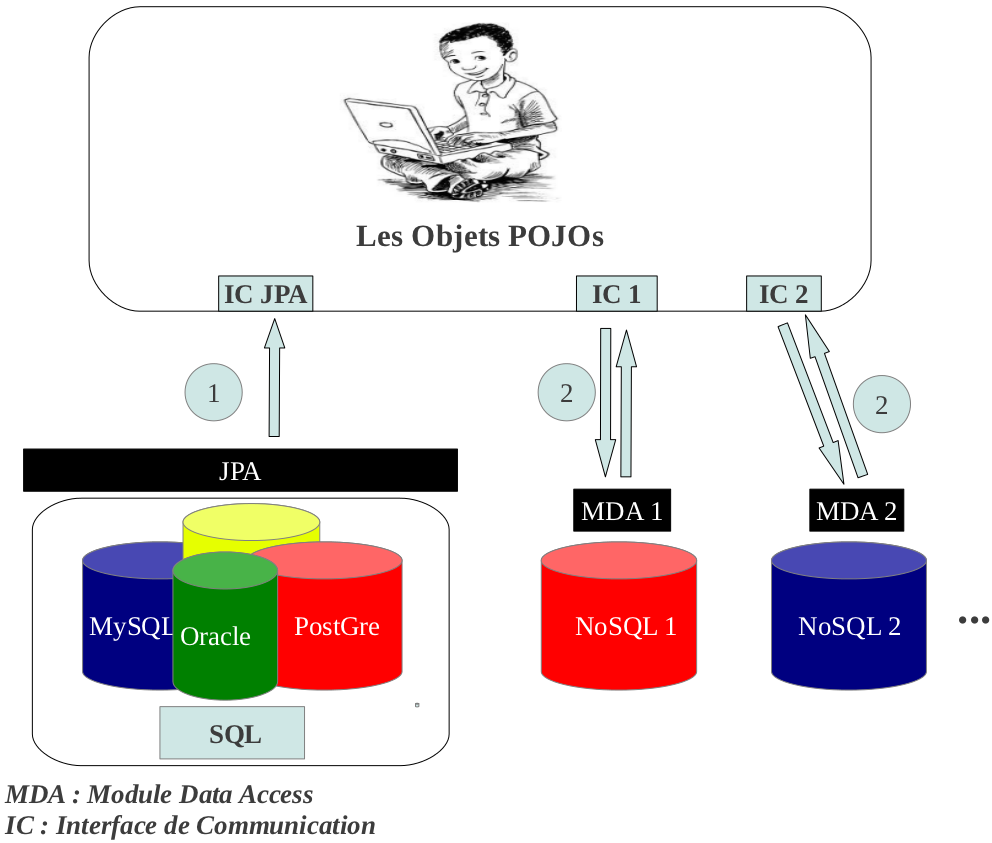
\includegraphics[scale=0.2]{\DIR/img/spring.png}	
        \caption{Possibilité d'échange \textsf{SQL/NoSQL} avec \textsf{spring}}
	\label{spring}
\end {figure}


\section{Système de Rootage intelligent entre \textsf{SQL} et \textsf{NoSQL}}
Il n'y vraiment pas grand chose à ce sujet. Ce qui ressort à chaque fois ce sont les motivations pour adopter le \textsf{NoSQL} qui sont: quantités de données et environnement distribué à fort trafic.

